\documentclass[../main.tex]{subfiles}

\graphicspath{{../images/}}

\begin{document}
\pagestyle{fancy}
\lhead{Lecture 1: 8/27/24}
\chead{Chapter 1}
\rhead{PHYS 421}

\section{Vector Analysis}
\barh 

\subsection{What is a Vector?}

In type we use boldface $\vb A = \abs{\vb A} \vu A$, where we we can do some simple operations as such:

\begin{itemize}
    \item Adding and Subtraction: $\vb A \pm \vb B = \vb C$ or aligning the head to the tail
    \item Multiplication:
    \begin{itemize}
        \item Scalar: $\vb A \to 2 \vb A$
        \item Dot Product: $\vb A \cdot \vb B = \vb B \cdot \vb A = AB \cos\theta$
        \item Cross Product: $\vb A \cross \vb B = AB \sin\theta$, and $\vb B \cross \vb A = -(\vb A \cross \vb B)$
    \end{itemize}
\end{itemize}

\paragraph*{Components of a Vector}

In 3D space, we often use the familiar Cartesian coordinates, e.g.
\[\vb A = A_x \vu x + A_y \vu y + A_z \vu z\]
and we can add components by adding the components:
\[\vb A + \vb B = (A_x + B_x) \vu x + (A_y + B_y) \vu y + (A_z + B_z) \vu z\]
and likewise for subtraction. For the dot product:
\[\vb A \cdot \vb B = A_x B_x + A_y B_y + A_z B_z\]
or more shortly
\[= \sum_{i,j} A_i B_j \delta_{ij}\]
where $\delta_{ij}$ is the Kronecker delta. The cross product is a bit trickier\dots
\[\vb A \cross \vb B = \begin{vmatrix}
    \vu x & \vu y & \vu z \\
    A_x & A_y & A_z \\
    B_x & B_y & B_z
\end{vmatrix}
= (A_y B_z - A_z B_y) \vu x - (A_x B_z - A_z B_x) \vu y + (A_x B_y - A_y B_x) \vu z\]
This can also be written in short form using the Levi-Civita symbol (look it up)

\paragraph*{Scalar triple product}
\[\vb A \cdot (\vb B \cross \vb C) = \vb B \cdot (\vb C \times \vb A) = \vb C \cdot (\vb A \cross \vb B)\]
This is the also the volume of the parallelepiped formed by the three vectors. NOTE that
\[\cancel{(\vb A \cdot \vb B) \cross \vb C}\]
since you can't cross a scalar with a vector.

\paragraph*{Vector triple product}
\[\vb A \cross (\vb B \cross \vb C) = \vb B(\vb A \cdot \vb C) - \vb C(\vb A \cdot \vb B)\]
Using the BAC-CAB rule. 

\paragraph*{Some important vectors}
We define a position vector 
\[\vb r = x \vu x + y \vu y + z \vu z = r \vu r\]
where the unit vector is
\[\vu r \equiv \frac{\vb r}{r}, \quad r = \sqrt{x^2 + y^2 + z^2}\]
and an infinitesimal displacement vector
\[\dd{l} = \dd x \vu x + \dd y \vu y + \dd z \vu z\]

\subparagraph*{In EM}
we define a source point $\vb r'$ (e.g. a charge) and a field point $\vb r$ that give us the seperation vector
\[\boldscriptr = \vb r = \vb r'\]
with magnitude
\[\abs{\boldscriptr} = \abs{\vb r - \vb r'}\]
and unit vector
\[\vu r = \frac{\vb r - \vb r'}{\vb r - \vb r'}\]

\subsection{Differential Calculus}

And ordinary derivative $\dv{F}{x}$ is a change in $F(x)$ in $\dd x$
\[\dd F = \qt(\pdv{F}{x})\dd x\]
\dots geometrically, it's the slope

\paragraph*{Gradient}
for functions of 2 or more variables, generalize for $h(x,y)$
\[\dd h = \qt(\pdv{h}{x}) \dd x + \qt(\pdv{h}{y}) \dd y\]
it's a scalar so \(\dd h = (\grad h) \cdot (\dd l)\) where
\[\grad h = \pdv{h}{x} \vu x + \pdv{h}{y} \vu y \]

\subparagraph*{In 3D}
\[\grad T = \pdv{T}{x} \vu x + \pdv{T}{y} \vu y + \pdv{T}{z} \vu z\]
If $\grad u = 0$, we are at an extremum (max, min, or shoulder/saddle point)
Rewriting:
\[\grad T = \qt(\vu x \pdv{x} + \vu y \pdv{y} + \vu z \pdv{z}) T(x,y,z)\]
wehere we can assume the $\nabla$ as an ``operator'' acting on $T$:
\begin{enumerate}
    \item Scalars like $T$: $\grad T$, ``grad T'', generalized slope
    \item Dot product on $\vb V$: $\div \vb V$, ``divergence'' or ``div''
    \item Cross product : $\curl \vb V$, ``curl'' or ``rotatation''
\end{enumerate}
\paragraph*{Divergence}
\begin{figure*}[ht]
    \centering
    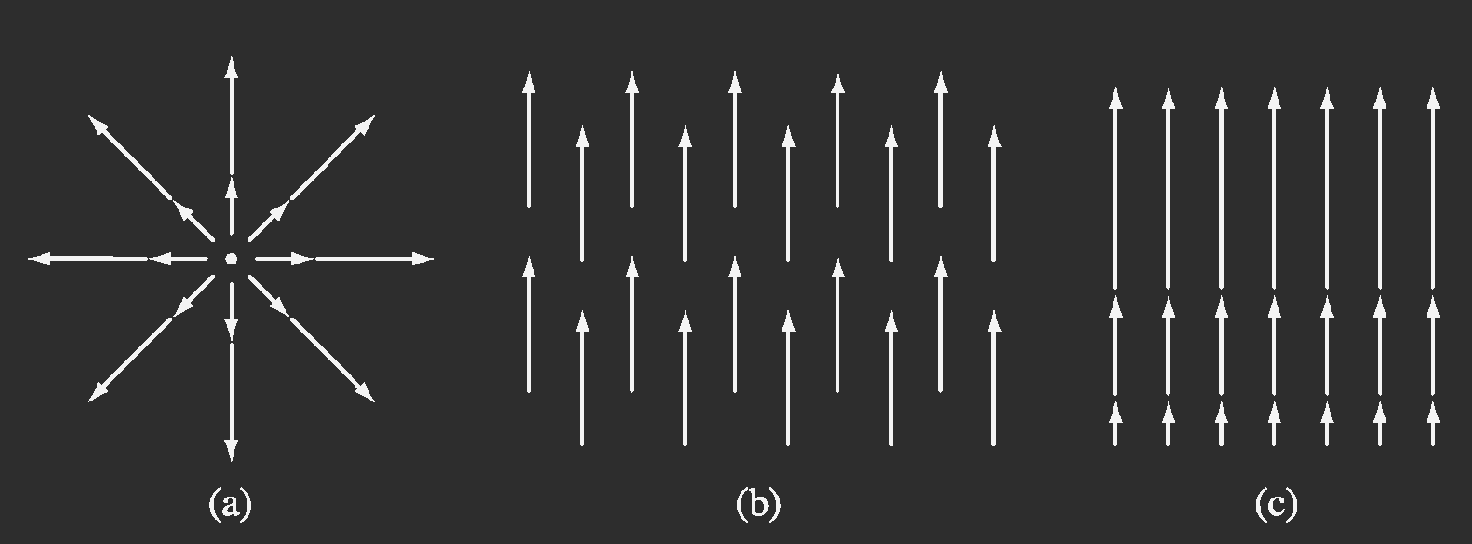
\includegraphics[width=0.5\textwidth]{fig1.1.png}
    \caption{Divergence of field lines}
\end{figure*}
From the Figure, we can see that (a) \& (c) diverges, and (b) does not.
\subparagraph*{Geometrical Interpretation:} Sources of positive divergence is a source or ``faucet'',
and negative divergence is a sink or ``drain''.

\paragraph*{Curl }
\[\curl \vb V = \begin{vmatrix}
    \vu x & \vu y & \vu z \\
    \pdv{x} & \pdv{y} & \pdv{z} \\
    V_x & V_y & V_z
\end{vmatrix}\]
E.g. for $\vb V = -y \vu x + x \vu y$, $\curl \vb V = 2 \vu z$.

\paragraph*{Combining Multiple Operations}
Two ways to get scalar from two functions:
\[fg \qor \vb A \cdot \vb B \]
Two ways to get vector from two functions:
\[f\vb A \qor \vb A \cross \vb B \]
And we have 3 `derivatives': div, grad, and curl.

Product rule: \[\partial_x (fg) = f \partial_x g + g \partial_x f\]

\begin{enumerate}
    \item[i] \(\grad(fg) = f \grad g + g \grad f\)
    \item[ii] \(\grad(\vb A \cdot \vb B) = \vb A \cross (\curl \vb B) + B \cross (\curl \vb A) + (\vb A \cdot \grad) \vb B + (\vb B \cdot \grad) \vb A\)
\end{enumerate}
\dots (see Griffiths for more)
\newpage
\lhead{Lecture 2: 8/29/24}

\paragraph*{Second Derivatives}

Combining $\grad, \div, \curl$

$\grad T$ is a vector

\begin{enumerate}
    \item[i] 
    \begin{align*}
        \div(\grad T) &= (\vu x \partial_x + \vu y + \partial_y + \vu z \partial_z) \cdot (\vu x \partial_x T + \vu y \partial_y T + \vu z \partial_z T) \\
        &= \partial_x^2 T + \partial_y^2 T + \partial_z^2 T \\
        &= \laplacian T
    \end{align*}
    \item[ii] $\curl (\grad T) = 0$
    \item[iii] $\grad(\div \vb v) = \dots$ ignored
    \item[iv] $\div(\curl \vb v) = 0$
    \item[v] $\curl(\curl \vb v) = \grad(\div \vb v) - \laplacian \vb v$
\end{enumerate}

\paragraph*{Integral Calculus:}

line, surface and volume integrals

\paragraph*{``Fundamental theorem for gradients''}

Start with a scalar $T(x,y,z)$: from $a \to b$, in small steps $\dd{T} = \div T \dd{\vb*\ell}$

Total change in $T$:
\begin{align*}
    \boxed{\int_a^b \dd T = \int_a^b \grad T \cdot \dd{\vb*\ell} = T(b) - T(a)} 
\end{align*}
This line integral is path independent but $\int_a^b \vb F \cdot \dd{\vb \ell}$ is \emph{not}!

\paragraph*{Divergence Theorem, ``Gauss' Theorem'', or ``Green's Theorem''}

\begin{align*}
    \boxed{
        \int_V (\div \vb v) \dd \tau = \oint_S \vb \vb v \cdot \dd{\vb a}
    }
\end{align*}
where $V$ is the volume enclosed by the surface $S$. The divergence of a field in a volume is equivalent to the flux of the field at the boundary or surface.

\subparagraph*{Geometrical Interpretation:} 

The ``source''(or faucet) should present a flux (or flow) out through the surface.

\paragraph*{Fundamental Theorem of Curls:} Stokes' Theorem
\begin{align*}
    \boxed{
        \oint_S (\curl \vb v) \cdot \dd{\vb a} = \oint_P \vb v \cdot \dd{\vb*\ell}
    }
\end{align*}
We have a 2D surfaces $S$ bounded by a closed 1D perimeter $P$.

In 3D, imagine a soap bubble in a wire frame. We can change the surface of the bubble by moving the wire frame and making almost making a bubble, but the perimeter that bounds the bubble is still the wireframe.

\paragraph*{Example:}
\begin{align*}
    \vb v = (2xz + 3y^2)\vu y + 4yz^2 \vu z
\end{align*}
On a surface $S$ square on the $y-z$ plane:
\begin{align*}
    \oint \vb v \cdot \dd{\vb*\ell} &= 
\end{align*}
RHS: We can split this into 4 integrals going counterclockwise around the square:
First
$ x = 0, z = 0, y: 0 \to 1$: $dx = dz = 0$
$\int_0^1 3y^2 \dd y = 1$

Second
$\int_0^1 4z^2 \dd z = 4/3$

Third: -1

Fourth: 0

Summing them all gives: $\oint \vb v \cdot \dd{\vb*\ell} = 4/3$

LHS:
The curl gives: $4z^2-2x, -(0-0), 2z$ so
\begin{align*}
    \oint(\curl \vb v) \cdot \vb{\dd \vb a} &= \oint 
\end{align*}
\dots

\subsection{Dirac Delta Function}
Considering a vector function
\begin{align*}
    \vb v = \frac{1}{r^2} \vu r
\end{align*}
[insert picture of field lines]

\begin{align*}
    \div \vb v &= \frac{1}{r^2} \pdv{r}(r^2 \frac{1}{r}) = 0
\end{align*}
The div theorem doesn't obviously tell what volume and surface to choose,
but we can choose a sphere of radius $R$ and its corresponding surface:
\begin{align*}
    \oint_S \vb v \cdot \dd{\vb a} &= \int \frac{1}{R^2} \vu r \cdot \vu r R^2 \sin\theta \dd\theta \dd\phi = 4\pi
\end{align*}
where the polar angle is $\theta: 0 \to \pi$ and the azimuthal angle is $\phi: 0 \to 2\pi$.

We think that the divergence is zero (thus the theorem does not hold), but we make a tiny mistake:

\paragraph*{}
$\div \vb v = 0$ everywhere except at the origin $r \to 0$

and we stumbled on the Dirac delta function:
\begin{align*}
    \delta(x) = \begin{cases}
        0 & x \neq 0 \\
        \infty & x = 0
    \end{cases}
    \qand \int_{-\infty}^{\infty} \delta(x) \dd x = 1
\end{align*}
where
\[\int f(x)\delta(x) \dd x = f(0)\]
Shifting the delta function:
\begin{align*}
    \delta(x - a) = \begin{cases}
        0 & x \neq a \\
        \infty & x = a
    \end{cases}
\end{align*}
so
\[\int f(x) \delta(x - a) \dd x  = f(a)\]
Multiplying by a constant:
\[\delta(kx) = \frac{1}{\abs{k}} \delta(x)\]
Generalizing to 3D:
\[\delta^3(\vb r) = \delta(x) \delta(y) \delta (z)\]

\paragraph*{Examples:}
\[\int_V (\div (\vb v)) \dd\tau = \int 4\pi \delta^3(\vb r) = 4\pi\]
and
\[\div (\frac{\vu\scriptr}{\boldscriptr^2}) = 4\pi \delta^3(\boldscriptr)\]
\end{document}